\iffalse
\let\negmedspace\undefined
\let\negthickspace\undefined
\documentclass[journal,12pt,twocolumn]{IEEEtran}
\usepackage{cite}
\usepackage{amsmath,amssymb,amsfonts,amsthm}
\usepackage{algorithmic}
\usepackage{circuitikz}
\usepackage{graphicx}
\usepackage{textcomp}
\usepackage{xcolor}
\usepackage{txfonts}
\usepackage{listings}
\usepackage{enumitem}
\usepackage{mathtools}
\usepackage{gensymb}
\usepackage{comment}
\usepackage[breaklinks=true]{hyperref}
\usepackage{tkz-euclide} 
\usepackage{listings}
\usepackage{gvv}                                        
\def\inputGnumericTable{}                                 
\usepackage[latin1]{inputenc}                                
\usepackage{color}                                            
\usepackage{array}                                            
\usepackage{longtable}                                       
\usepackage{calc}                                             
\usepackage{multirow}                                         
\usepackage{hhline}                                           
\usepackage{ifthen}                                           
\usepackage{lscape}
\newtheorem{theorem}{Theorem}[section]
\newtheorem{problem}{Problem}
\newtheorem{proposition}{Proposition}[section]
\newtheorem{lemma}{Lemma}[section]
\newtheorem{corollary}[theorem]{Corollary}
\newtheorem{example}{Example}[section]
\newtheorem{definition}[problem]{Definition}
\newcommand{\BEQA}{\begin{eqnarray}}
\newcommand{\EEQA}{\end{eqnarray}}
\newcommand{\define}{\stackrel{\triangle}{=}}
\theoremstyle{remark}
\newtheorem{rem}{Remark}
\begin{document}

\bibliographystyle{IEEEtran}
\vspace{3cm}
\title{NCERT Question 11.9.3.9}
\author{EE23BTECH11019 - Faisal Imtiyaz $^{*}$% <-this % stops a space
}
\maketitle
\newpage
\bigskip

\renewcommand{\thefigure}{\arabic{figure}}
\renewcommand{\thetable}{\arabic{table}}


\vspace{3cm}
\textbf{Question:}
The R-L circuit with $R=10 k\Omega$ and $L=1 mH$ is excited by a step current $I_0u(t)$. At $t=0^-$, there is a current $I_L=I_0/5$ flowing through the inductor. The minimum time taken for the current through the inductor to reach $99\%$ of its final value is $\ldots \mu s$
(rounded off to two decimal places).\\
\begin{figure}[h!]
    \centering
    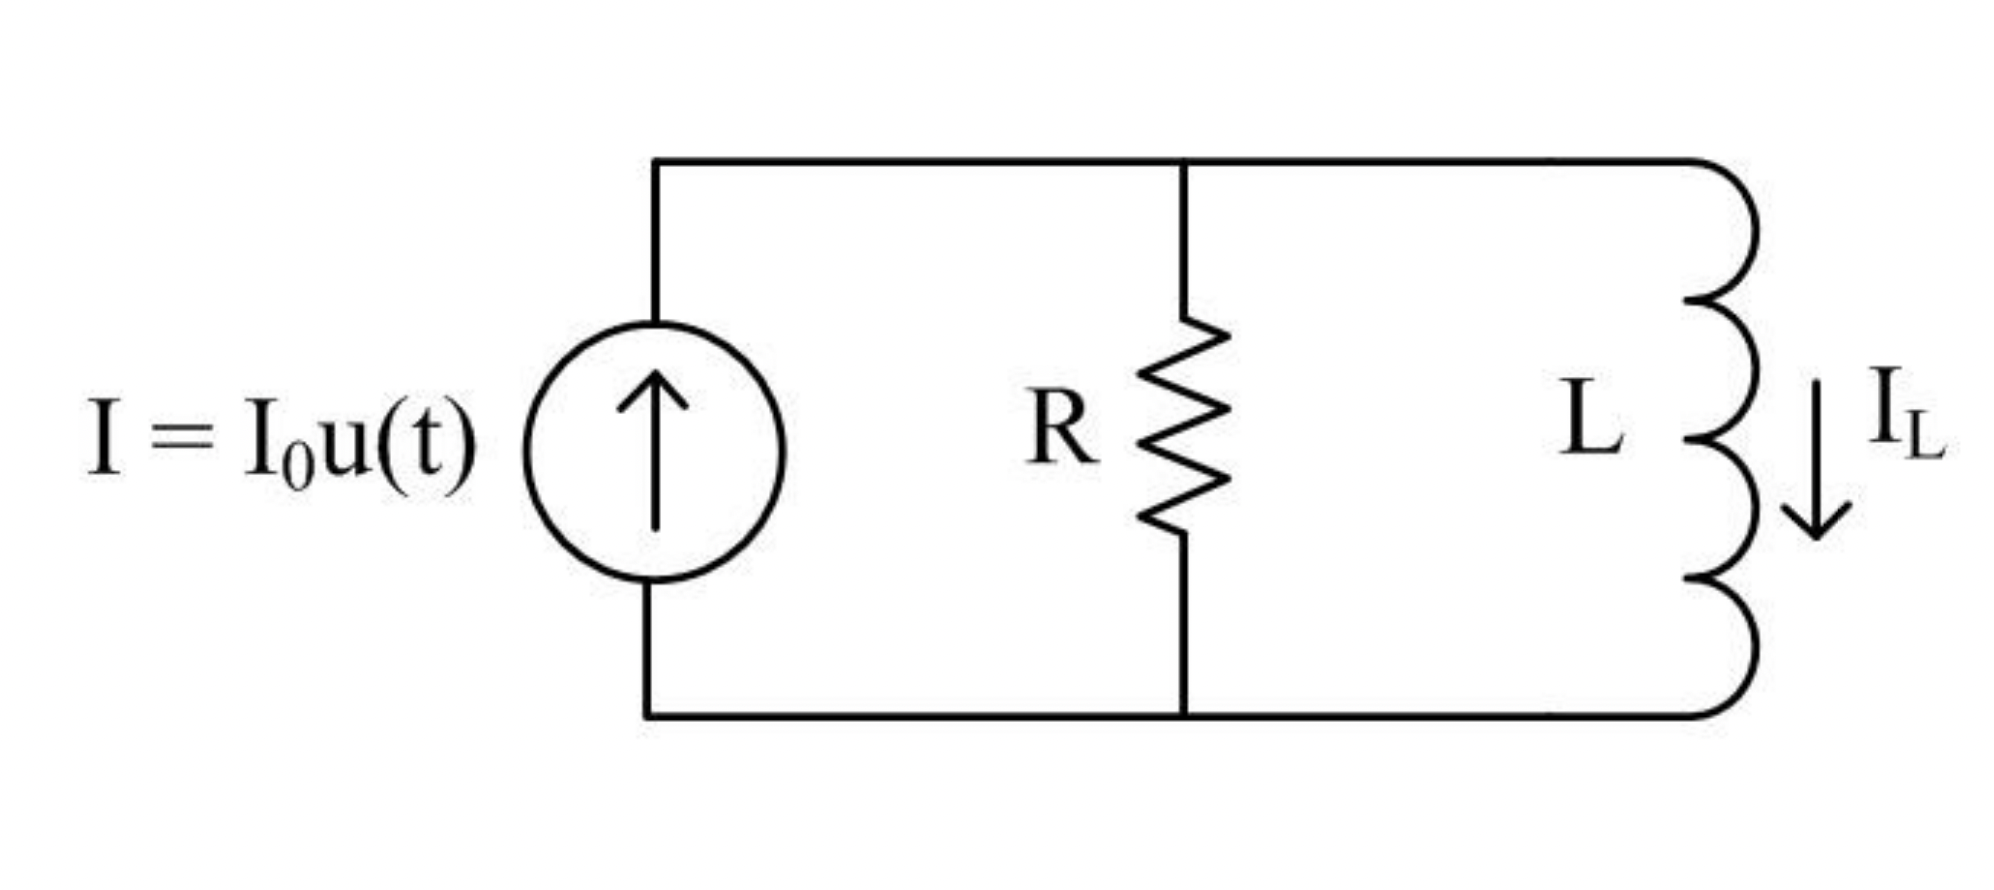
\includegraphics[width=0.8\columnwidth]{question.png}
\end{figure}
\textbf{Solution:}\\
\fi
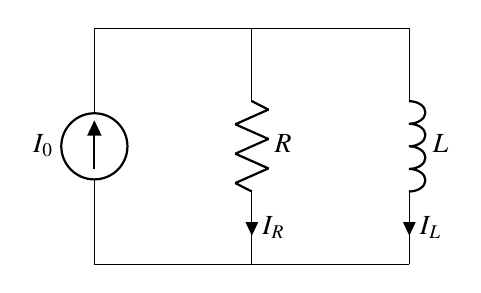
\begin{tikzpicture}[american]
    % Draw components
    \draw (0,0) to[american current source, l=$I_0$] (0,3); % Current source
    \draw (0,3) -- (2,3) to[R, l=$R$, i=$I_R$] (2,0); % Resistor
    \draw (2,3) -- (4,3) to[L, l=$L$, i=$I_L$] (4,0); % Inductor
    \draw (4,0) -- (0,0); % Connection between resistor and inductor
\end{tikzpicture}

\begin{table}[htbp]
    \centering
    \def\arraystretch{1.5}
    \begin{tabular}{|p{2.5cm}|p{3cm}|}
        \hline
        \textbf{Transform} & \textbf{Signal} \\
        \hline
        $\frac{1}{s(s+a)}$ & $\frac{1}{a}(1-e^{-at})$ \\
        \hline
        $\frac{1}{s+a}$ & $e^{-at}$ \\
        \hline
    \end{tabular}
    \caption{Inverse Laplace transform pairs}
    \label{laplace-transform-pairs-table}
\end{table}

\begin{align}
    I_0u\brak{t} &= I_R + I_L
\end{align}
From KVL, we have:
\begin{align}
    (\frac{I_0}{s} -I_L\brak{s})R - L(sI_L\brak{s} - I_L\brak{0^-}) &=0
\end{align}
After Simplyfying we have:
\begin{align}
    I_L\brak{s} &= \frac{ I_0R +LsI_L\brak{0^-}}{s(R+Ls)}\\
    I_L\brak{s} &= \frac{I_0R}{L}\frac{1}{s(s+\frac{R}{L})} + \frac{I_0}{5}\frac{1}{\frac{R}{L}+s}
\end{align}
From \tabref{laplace-transform-pairs-table}, we have:
\begin{align}
    I_L\brak{t} & = \frac{I_0R}{L} \sbrak{\frac{1}{\frac{R}{L}}(1-e^{-\frac{R}{L}t})} + \frac{I_0}{5}e^{-\frac{R}{L}}\\
    I_L\brak{t} &= I_0 -\frac{4}{5}I_0e^{-\frac{R}{L}t}\\
    I_L\brak{t} &= I_0 -\frac{4}{5}I_0e^{-10^{7}t}\\
    \lim_{t \to \infty} I_L\brak{t} &= I_0
\end{align}
Now time when current in inductor is $99\%$ of its final value is given by:
\begin{align}
    0.99I_0 &= I_0 -\frac{4}{5}I_0e^{-\frac{R}{L}t}\\
    0.01I_0 &= \frac{4}{5}I_0e^{-\frac{R}{L}t}\\
    t &= \frac{L}{R}\ln(80)\\
    t &= 10^{-7}\ln(80) \mu s\\
    t &= 0.43 \mu s
\end{align}
\begin{figure}[ht!]
	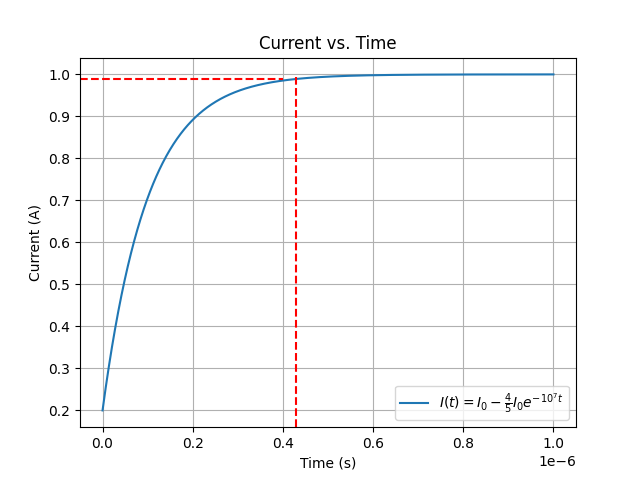
\includegraphics[width=\columnwidth]{2023/IN/47/plots/Figure_1.png}
	% \caption{Plot of $y(n)$ for $a=0.7$}
\end{figure}

  
% \end{document}